\section{Introduction}
\label{sec:intro}
Many long-context applications ask different questions about a stable collection of manuals, repositories, or conversation histories. Retrieval reduces the text processed for each question, but a conventional decoder still runs every selected token through every layer \citep{rag,retrievallong}. Each retrieval of the same passage therefore repeats the computation that encodes its content. Reusing that encoding would let the model begin from an already processed representation of the passage.

\textbf{Our key insight is to exploit the semantic-encoder role of early transformer layers.} These layers transform tokens into contextual representations, and semantic information can already be read from intermediate states before the final next-token readout. This motivates a functional decomposition: a lower-layer encoder constructs reusable document representations, while an upper-layer reader consumes the selected representations together with a query. Caching at their boundary lets future queries reuse document encoding and execute only the remaining document layers. Figures~\ref{fig:teaser} and~\ref{fig:arch} illustrate this encoder--cache--reader view.

This interface lies between storing raw text, which requires full-depth encoding on every query, and storing full-depth chunk KV, which prepays more computation with a larger persistent object \citep{promptcache,cacheblend,turborag}. MidCache caches the output of a chosen encoder prefix and leaves the remaining blocks available to process retrieved chunks together.

MidCache implements this insight through a \writepass{}--\readpass{} interface. Document \writepass{} independently encodes each chunk through the lower $j$ layers and persists its residuals. Online \readpass{} retrieves a bounded set of chunks, assembles their cached states with the encoded query, and continues through layers $[j{:}L)$. A self-distilled suffix adapter learns to read independently encoded states while leaving the backbone frozen. At $j=0$, the same selected tokens pass through all layers, providing a fixed-evidence reference for the saved encoding work.

\begin{figure}[htbp]
\centering
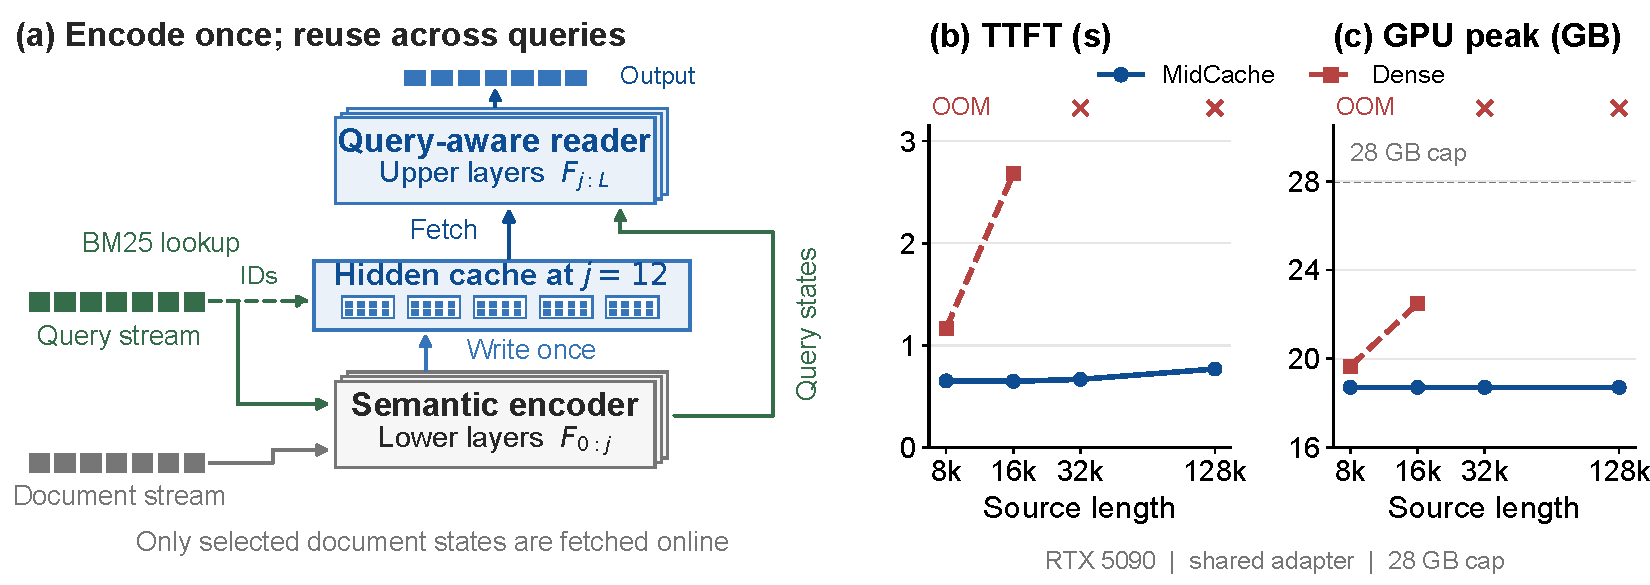
\includegraphics[width=\linewidth]{figures/teaser.pdf}
\caption{\textbf{A hidden cache between two parts of the LLM.} (a) The lower layers serve as a semantic encoder: their document states are cached once and reused by the upper reader. BM25 selects chunk IDs; only selected states are fetched. The query is also encoded before upper-layer continuation. (b--c) RTX 5090 measurements from Table~\ref{tab:infra}. TTFT includes retrieval, fetch, and query Write, but excludes document Write. GPU peaks include weights. Crosses mark actual Dense OOMs under the 28 GB allocator cap, without numerical values or extrapolation.}
\label{fig:teaser}
\end{figure}


We test both parts of this argument: whether intermediate states carry useful semantic information, and whether a decoder can reuse them efficiently. Layerwise probes motivate the encoder view; continuation checks, split-depth tests, and same-evidence comparisons evaluate the cache interface itself. MidCache reduces selected-pack prefill time on Qwen3-8B, with a measurable RULER accuracy cost. Independently encoded chunks also lose cross-chunk context, making quality task-dependent and motivating suffix adaptation and Write-context controls. The encoder view is a reusable computation boundary, not a claim that semantic processing ends at a universal layer.

Deployment depends on reuse. Residuals are smaller than full-depth KV but larger than token IDs, and construction must be amortized over future queries. Accounting for Write, fetch, Read, and decode shows how source length, output length, and storage placement affect this crossover. Tests with latency-calibrated chunk budgets then assess whether spending the saved computation on additional evidence improves quality.

\paragraph{Contributions.}
\begin{itemize}[leftmargin=1.3em,itemsep=2pt,topsep=3pt]
\item \textbf{A semantic-encoder cache.} MidCache turns lower-layer document representations into persistent memory and reuses them through the decoder's own upper layers.
\item \textbf{An adapted reader and a testable interface.} Suffix self-distillation, continuation checks, and fixed-evidence context/depth controls establish how independently encoded states can be read and where fidelity is lost.
\item \textbf{Measured conditions for useful reuse.} Repeated-query accounting and latency-calibrated budget comparisons quantify both amortization and the cases where raw replay remains preferable.
\end{itemize}
\FloatBarrier
